%%%%%%%%%%%%%%%%%%%%%%%%%%%%%%%%%%%%%%%%%%%%%%%%%%%%%%%%%%%%%%%%%%%%%%%%%%%%%%
% CS110: Introduction to Computing
% Copyright 2015 Pejman Ghorbanzade <mail@ghorbanzade.com>
% Creative Commons Attribution-ShareAlike 4.0 International License
% https://github.com/ghorbanzade/UMB-CS110-2015S/blob/master/LICENSE
%%%%%%%%%%%%%%%%%%%%%%%%%%%%%%%%%%%%%%%%%%%%%%%%%%%%%%%%%%%%%%%%%%%%%%%%%%%%%%

\def \topDirectory {.}
\def \texDirectory {\topDirectory/src/main/tex}

\documentclass[12pt,letterpaper,twoside]{article}
\usepackage{\texDirectory/template/style/directives}
\usepackage{\texDirectory/template/style/assignment}
%%%%%%%%%%%%%%%%%%%%%%%%%%%%%%%%%%%%%%%%%%%%%%%%%%%%%%%%%%%%%%%%%%%%%%%%%%%%%%
% CS110: Introduction to Computing
% Copyright 2015 Pejman Ghorbanzade <mail@ghorbanzade.com>
% Creative Commons Attribution-ShareAlike 4.0 International License
% https://github.com/ghorbanzade/UMB-CS110-2015S/blob/master/LICENSE
%%%%%%%%%%%%%%%%%%%%%%%%%%%%%%%%%%%%%%%%%%%%%%%%%%%%%%%%%%%%%%%%%%%%%%%%%%%%%%

\course{id}{CS110}
\course{name}{Introduction to Computing}
\course{venue}{Tue/Thu, 5:30 PM - 6:45 PM}
\course{semester}{Spring 2015}
\course{department}{Department of Computer Science}
\course{university}{University of Massachusetts Boston}

\instructor{name}{Pejman Ghorbanzade}
\instructor{title}{}
\instructor{position}{Student Instructor}
\instructor{email}{pejman@cs.umb.edu}
\instructor{phone}{617-287-6419}
\instructor{office}{S-3-124B}
\instructor{office-hours}{Tue/Thu 19:00-20:30}
\instructor{address}{University of Massachusetts Boston, 100 Morrissey Blvd., Boston, MA}


\begin{document}

\doc{title}{Quiz 1(a)}
\doc{date-pub}{Feb 24, 2015 at 01:00 PM}
\doc{date-due}{Feb 24, 2015 at 11:00 PM}
\doc{points}{4}

\prepare{header}

\section*{Question 1}

Meet, from left to right, Joe, William, Jack and Averell, villains of our childhood that go by the name of the Dalton brothers. These inseparable brothers have a special rule among themselves. They always stand in order of their height.

Write a program \texttt{TheDaltons.java} that takes names of the brothers as command-line arguments and prints \texttt{false} unless the order in which arguments are given follows \textit{The Dalton Rule}.

Example:\\
\texttt{\% java TheDaltons Joe William Jack Averell > true}\\
\texttt{\% java TheDaltons Averell Jack William Joe > true}\\
\texttt{\% java TheDaltons Averell William Joe Jack > false}

\begin{figure}[H]\centering
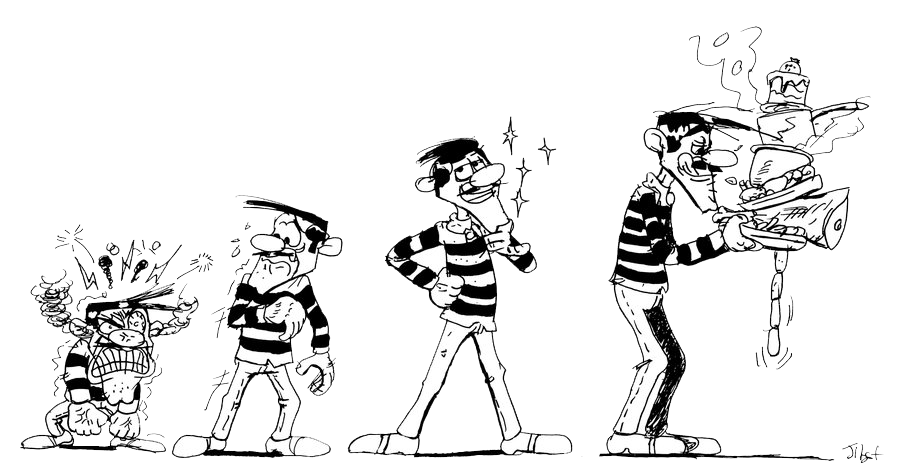
\includegraphics{\texDirectory/template/images/daltons.png}
\caption{The Dalton Brothers}
\end{figure}

\section*{Question 2}

Matthew and John are playing backgammon and they hate rolling the two dice each turn, over and over again.

\begin{enumerate}
\item Write a program \texttt{Dice1.java} that gives two random integer numbers from one to six each time it is executed.
\item Upgrade your program to \texttt{Dice2.java} such that it takes an integer number as command-line argument and generates two random integer values in the range of one to given integer number.
\end{enumerate}

\prepare{footer}

\end{document}
